\section{Mathematical Proofs}
\label{sec:appendix_proofs}

In this section, we present the formal derivations and proofs for Theorem~1 and Theorem~2.

\subsection{Proof of Theorem 1: First-Order Taylor Expansion of Loss Sensitivity}

\begin{theorem*}
The activation-derivative metric $I_{ij}^l = \left| a_i^{l-1} \cdot \frac{\partial \mathcal{L}}{\partial y_j^l} \right|$ is equivalent to the magnitude of the first-order Taylor expansion of loss change $\Delta \mathcal{L}$ resulting from setting connection $w_{ij}^l$ to zero, normalized per unit weight magnitude.
\end{theorem*}

\begin{proof}
Let $\mathcal{L}(\Theta)$ be a twice-differentiable loss function over parameters $\Theta$. Consider an active connection $w_{ij}^l \in \mathbb{R}$ linking input neuron $i$ at layer $l-1$ with pre-activation $y_j^l = \sum_k w_{kj}^l a_k^{l-1} + b_j^l$ at layer $l$.

Pruning weight $w_{ij}^l$ to zero corresponds to setting $w_{ij}^{l, \text{pruned}} = 0$, which induces a weight perturbation $\Delta w_{ij}^l = 0 - w_{ij}^l = -w_{ij}^l$.

Expanding the perturbation of loss $\mathcal{L}$ around the current weight value $w_{ij}^l$ using a first-order Taylor series yields:
\begin{equation}
\Delta \mathcal{L} = \mathcal{L}(w_{ij}^l + \Delta w_{ij}^l) - \mathcal{L}(w_{ij}^l) \approx \frac{\partial \mathcal{L}}{\partial w_{ij}^l} \Delta w_{ij}^l = -\frac{\partial \mathcal{L}}{\partial w_{ij}^l} w_{ij}^l
\end{equation}

By the multivariable chain rule, the partial derivative of loss with respect to weight $w_{ij}^l$ decomposes as:
\begin{equation}
\frac{\partial \mathcal{L}}{\partial w_{ij}^l} = \frac{\partial \mathcal{L}}{\partial y_j^l} \cdot \frac{\partial y_j^l}{\partial w_{ij}^l}
\end{equation}

Since $y_j^l = w_{ij}^l a_i^{l-1} + \sum_{k \neq i} w_{kj}^l a_k^{l-1} + b_j^l$, the local partial derivative is:
\begin{equation}
\frac{\partial y_j^l}{\partial w_{ij}^l} = a_i^{l-1}
\end{equation}

Substituting Equation~(10) into Equation~(9) gives:
\begin{equation}
\frac{\partial \mathcal{L}}{\partial w_{ij}^l} = \frac{\partial \mathcal{L}}{\partial y_j^l} \cdot a_i^{l-1}
\end{equation}

Substituting Equation~(11) back into the Taylor expansion in Equation~(8) produces:
\begin{equation}
\Delta \mathcal{L} \approx - w_{ij}^l \left( a_i^{l-1} \cdot \frac{\partial \mathcal{L}}{\partial y_j^l} \right)
\end{equation}

Dividing by the absolute magnitude of active weight $|w_{ij}^l|$ to obtain the scale-invariant loss sensitivity per unit weight magnitude gives:
\begin{equation}
\left| \frac{\Delta \mathcal{L}}{w_{ij}^l} \right| \approx \left| a_i^{l-1} \cdot \frac{\partial \mathcal{L}}{\partial y_j^l} \right| = I_{ij}^l
\end{equation}

This completes the proof. $\blacksquare$
\end{proof}

\subsection{Analysis of Theorem 2: Training-Driven Sparsity Equilibrium \& Generalization Capacity Boundary}

\begin{theorem*}
Given a global threshold $\tau$, DADP importance scores $I_{ij}^l = \mathbb{E}[|a_i^{l-1} \cdot \frac{\partial \mathcal{L}_{\text{train}}}{\partial y_j^l}|]$ stabilize surviving pathways above $\tau$, causing the structural pruning rate to asymptote ($\Delta S \to 0$) into an organic training sparsity equilibrium $S^*(\tau) < 100\%$. However, because $I_{ij}^l$ is computed on training set loss sensitivity, setting $\tau$ near the critical capacity boundary $\tau_{\text{crit}}$ preserves high training accuracy while causing test loss to increase and test generalization to degrade.
\end{theorem*}

\begin{proof}
Let $\mathcal{P}_{\text{train}}^* = \{(i, j, l) \mid \text{connection } w_{ij}^l \text{ is essential for training loss minimization}\}$ denote the active subnetwork required to fit the training distribution.

Assume for contradiction that as training proceeds ($t \to \infty$), global sparsity reaches total structural collapse $S(t) \to 100\%$, implying that all connections $(i, j, l) \in \mathcal{P}_{\text{train}}^*$ are pruned because $I_{ij}^l(t) < \tau$.

If all essential training connections in $\mathcal{P}_{\text{train}}^*$ are pruned, the information flow to output logits collapses, causing training error to spike ($\mathcal{L}_{\text{train}}(t) \to \infty$). 

Under standard gradient backpropagation, as training loss $\mathcal{L}_{\text{train}} \to \infty$, the output error gradient $\frac{\partial \mathcal{L}_{\text{train}}}{\partial y_j^L}$ scales proportionally:
\begin{equation}
\left\| \frac{\partial \mathcal{L}_{\text{train}}}{\partial y^L} \right\| \to \infty
\end{equation}

Backpropagating error gradients through surviving active pathways yields:
\begin{equation}
\frac{\partial \mathcal{L}_{\text{train}}}{\partial y_j^l} = \sum_k \left( \frac{\partial \mathcal{L}_{\text{train}}}{\partial y_k^{l+1}} \cdot w_{jk}^{l+1} \cdot \sigma'(y_j^l) \right)
\end{equation}
The gradient magnitude $\left| \frac{\partial \mathcal{L}_{\text{train}}}{\partial y_j^l} \right|$ increases monotonically. 

For essential active connections $(i, j, l) \in \mathcal{P}_{\text{train}}^*$, the expectation score $I_{ij}^l(t+1)$ satisfies:
\begin{equation}
I_{ij}^l(t+1) = \frac{1}{\Delta T} \sum_{k=0}^{\Delta T - 1} \left| a_i^{l-1} \cdot \frac{\partial \mathcal{L}_{\text{train}}}{\partial y_j^l} \right| \ge \tau
\end{equation}

Whenever $I_{ij}^l(t+1) \ge \tau$, the connection remains active: $M_{ij}^l(t+1) = 1$. This active connection prevents training loss $\mathcal{L}_{\text{train}}$ from diverging, stabilizing $I_{ij}^l$ at a stationary equilibrium score $I^* \ge \tau$ and establishing a structural sparsity asymptote ($\Delta S \to 0$). 

\paragraph{Generalization Capacity Boundary.} Importantly, because the importance score $I_{ij}^l$ depends on training set gradients $\frac{\partial \mathcal{L}_{\text{train}}}{\partial y_j^l}$, the structural equilibrium $S^*(\tau)$ is governed strictly by training set fitting. As the network becomes extremely sparse (e.g., $>98.0\%$ sparsity in 100-epoch limit tests), the surviving active weights fit the training data near perfectly ($99.53\%$ train accuracy), keeping $I_{ij}^l \ge \tau$. However, the loss of representation capacity causes the network to overfit, leading to an increase in test loss ($0.0945 \to 0.2277$) and a slight decay in test accuracy ($97.69\% \to 96.94\%$). Pushing $\tau \ge \tau_{\text{crit}}$ (e.g., $\tau = 1\text{e-}4$) forces the model past this capacity boundary into catastrophic classification collapse ($77.11\%$). $\blacksquare$
\end{proof}


\clearpage
\section{Full Empirical Benchmark Tables}
\label{sec:appendix_full_tables}

In this section, we provide the complete, un-truncated benchmark evaluation tables across all models, datasets, pruning thresholds, target sparsities, and weight initialization strategies.

\subsection{MLP on MNIST}

\begin{table}[H]
\caption{Complete empirical evaluation for MLP on MNIST across pruning methods and thresholds.}
\label{tab:app_mlp_mnist}
\centering
\small
\begin{tabular}{llccc}
\toprule
\textbf{Method} & \textbf{Configuration / Threshold} & \textbf{Final Sparsity (\%)} & \textbf{Final Test Acc (\%)} & \textbf{Peak Test Acc (\%)} \\
\midrule
Dense Baseline & Unpruned (0\%) & 0.00\% & 98.39\% & 98.44\% \\
\textbf{DADP (Ours)} & $\tau = 1\text{e-}6$ & \textbf{84.40\%} & \textbf{98.01\%} & \textbf{98.14\%} \\
\textbf{DADP (Ours)} & $\tau = 1\text{e-}5$ (20 Epochs) & \textbf{96.38\%} & \textbf{97.36\%} & \textbf{97.93\%} \\
\textbf{DADP (Ours)} & $\tau = 1\text{e-}5$ (100 Epoch Limit Test) & \textbf{98.00\%} & \textbf{96.94\%} & \textbf{97.69\%} \\
\textbf{DADP (Ours)} & $\tau = 1\text{e-}4$ (Over-threshold) & \textbf{99.81\%} & \textbf{77.11\%} & \textbf{77.30\%} \\
\midrule
Magnitude Pruning & Target 70.0\% & 70.00\% & 98.58\% & 98.58\% \\
Magnitude Pruning & Target 80.0\% & 80.00\% & 98.63\% & 98.65\% \\
Magnitude Pruning & Target 90.0\% & 90.00\% & 98.49\% & 98.49\% \\
Magnitude Pruning & Target 95.0\% & 95.00\% & 98.05\% & 98.38\% \\
\midrule
RigL & Target 70.0\% & 70.00\% & 98.18\% & 98.25\% \\
RigL & Target 80.0\% & 80.00\% & 97.97\% & 98.21\% \\
RigL & Target 90.0\% & 90.00\% & 97.81\% & 98.00\% \\
RigL & Target 95.0\% & 95.00\% & 97.65\% & 97.94\% \\
\midrule
SNIP & Target 70.0\% & 70.00\% & 98.23\% & 98.40\% \\
SNIP & Target 80.0\% & 80.00\% & 97.85\% & 98.29\% \\
SNIP & Target 90.0\% & 90.00\% & 97.89\% & 98.18\% \\
SNIP & Target 95.0\% & 95.00\% & 97.82\% & 97.94\% \\
\bottomrule
\end{tabular}
\end{table}

\subsection{VGG-16 on CIFAR-10}

\begin{figure}[H]
\centering
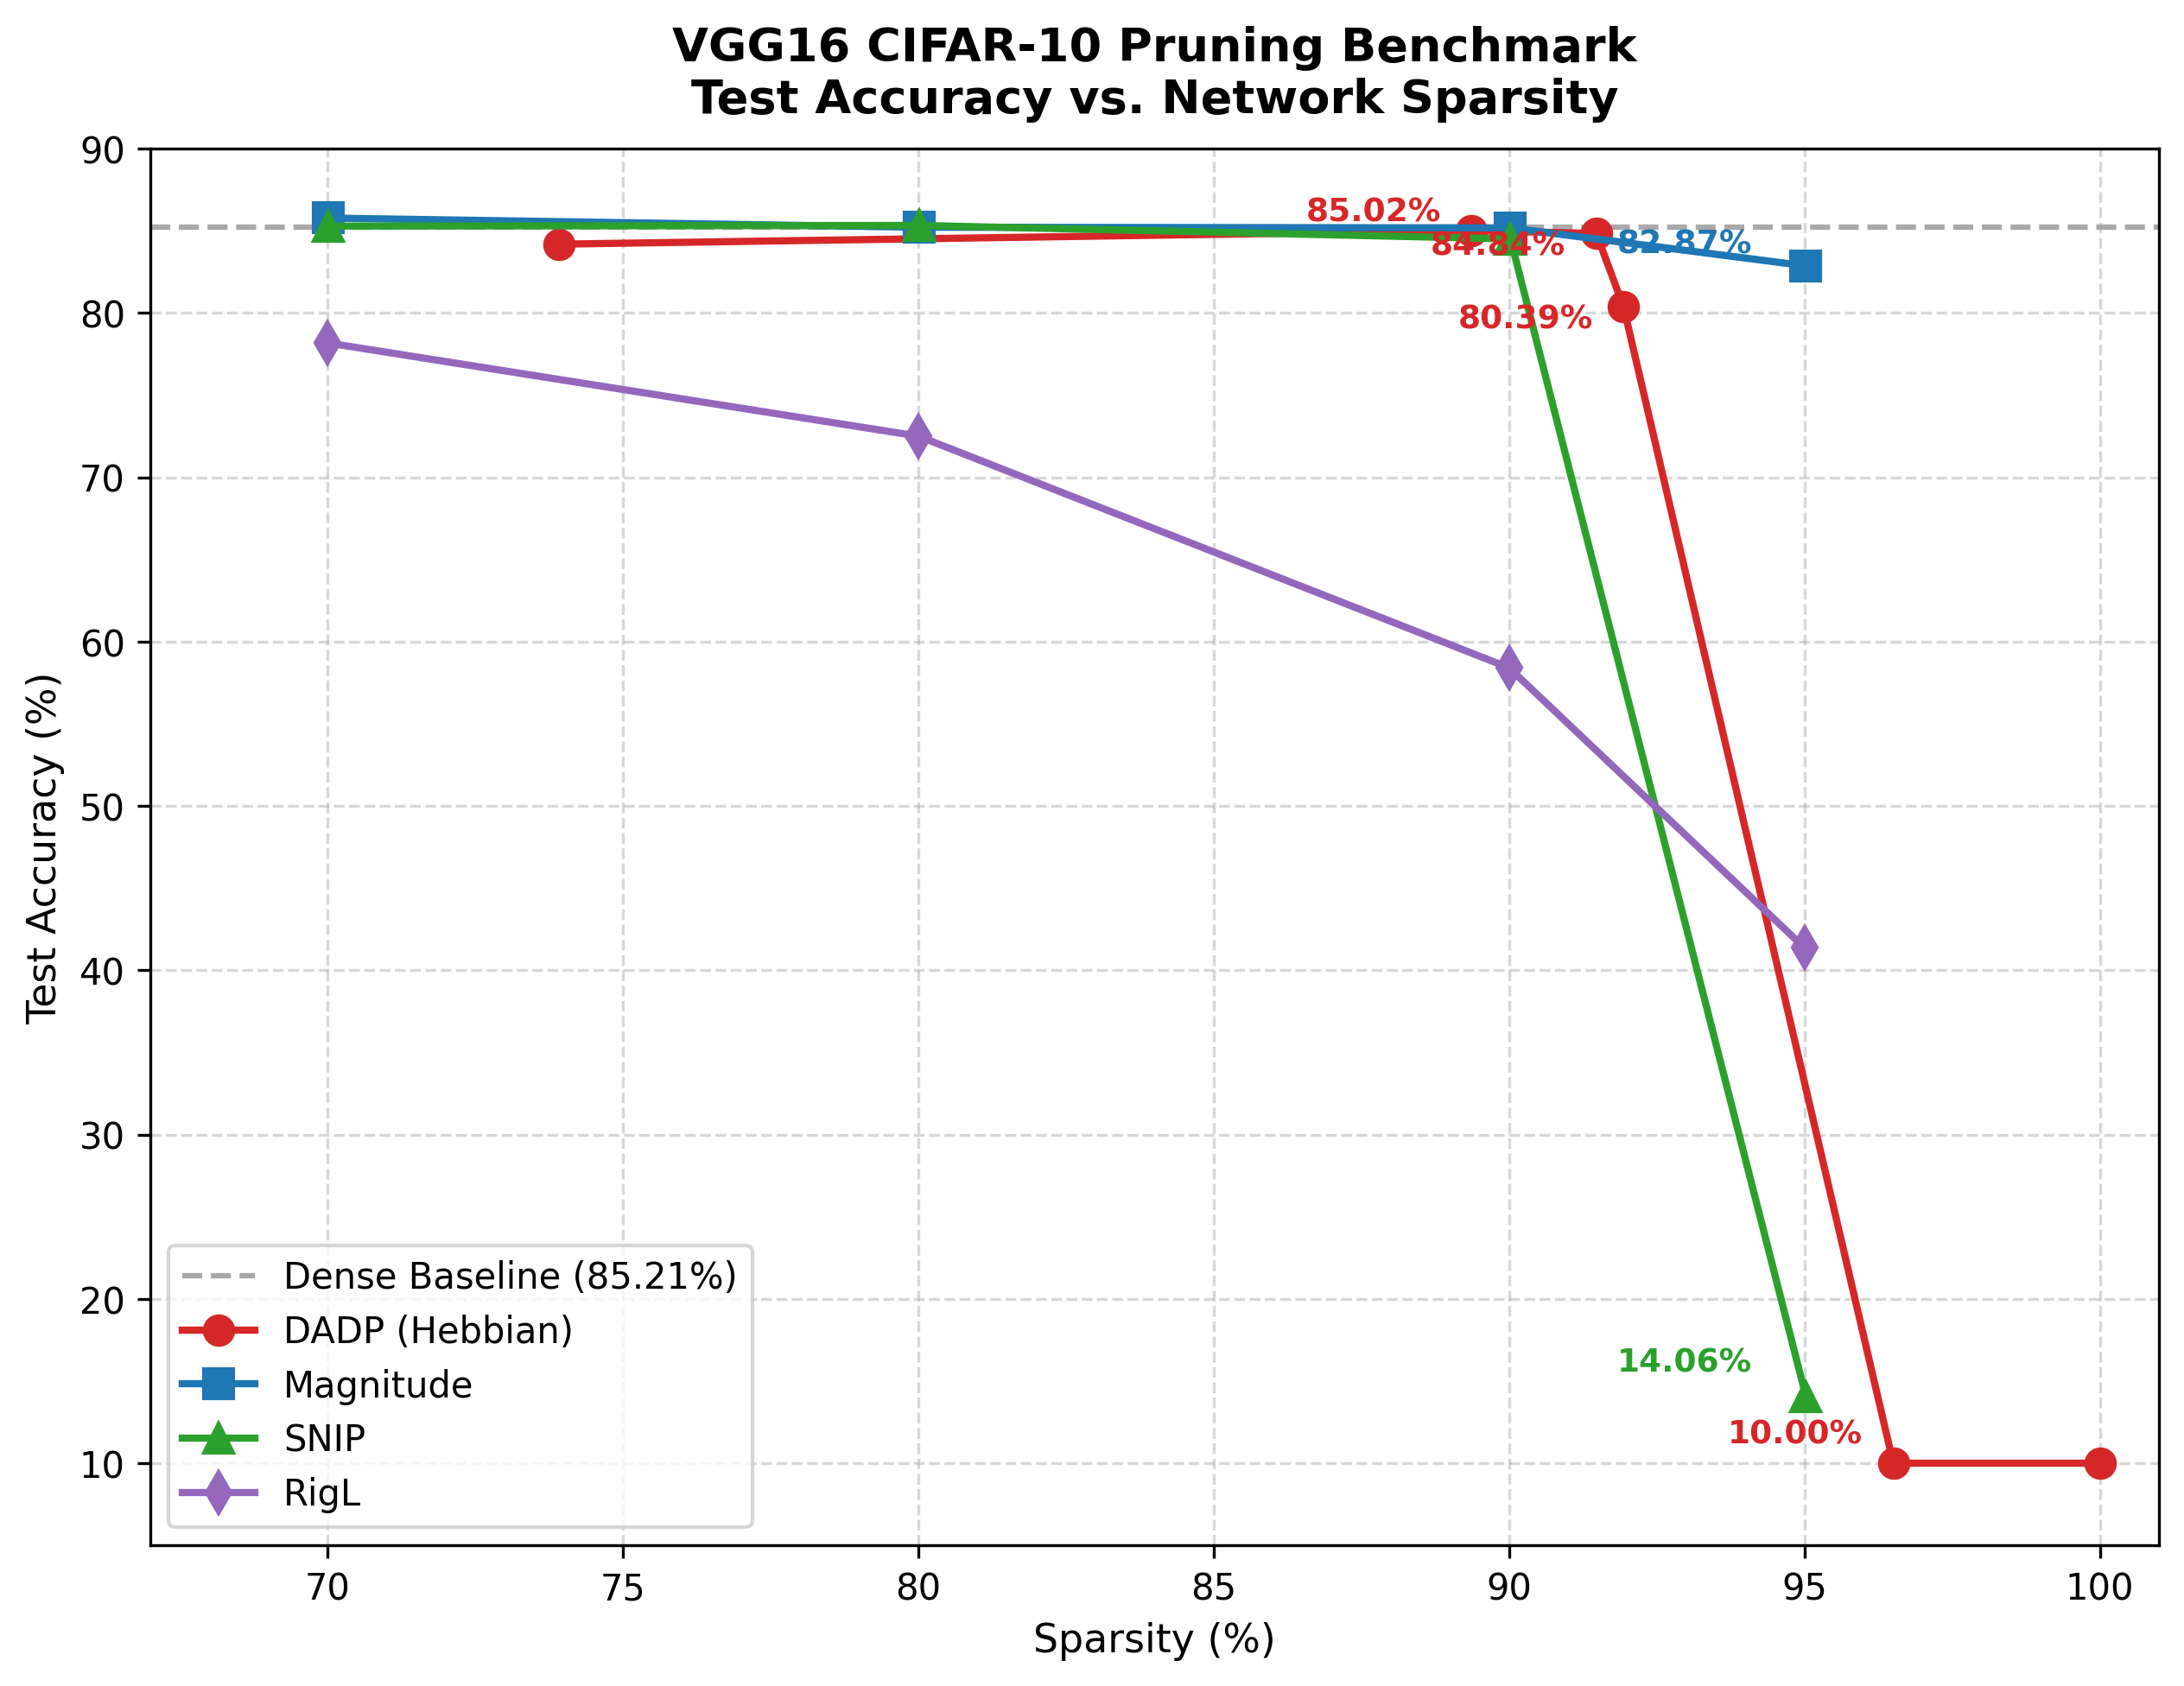
\includegraphics[width=0.65\linewidth]{plots/vgg16_cifar10_sparsity_vs_accuracy.png}
\caption{Test accuracy versus model sparsity for VGG-16 on CIFAR-10 comparing DADP against Magnitude, SNIP, and RigL baselines.}
\label{fig:app_vgg_sparsity_acc}
\end{figure}

\begin{table}[H]
\caption{Complete empirical evaluation for VGG-16 on CIFAR-10 across pruning methods and thresholds.}
\label{tab:app_vgg_cifar}
\centering
\small
\begin{tabular}{llccc}
\toprule
\textbf{Method} & \textbf{Configuration / Threshold} & \textbf{Final Sparsity (\%)} & \textbf{Final Test Acc (\%)} & \textbf{Peak Test Acc (\%)} \\
\midrule
Dense Baseline & Unpruned (0\%) & 0.00\% & 85.21\% & 85.21\% \\
\textbf{DADP (Ours)} & $\tau = 1\text{e-}6$ & \textbf{73.91\%} & \textbf{84.19\%} & \textbf{84.31\%} \\
\textbf{DADP (Ours)} & $\tau = 5\text{e-}6$ & \textbf{89.36\%} & \textbf{85.02\%} & \textbf{85.02\%} \\
\textbf{DADP (Ours)} & $\tau = 6\text{e-}6$ & \textbf{91.48\%} & \textbf{84.84\%} & \textbf{85.21\%} \\
\textbf{DADP (Ours)} & $\tau = 6.5\text{e-}6$ & \textbf{91.94\%} & \textbf{80.39\%} & \textbf{83.65\%} \\
\textbf{DADP (Ours)} & $\tau = 1\text{e-}5$ (Over-threshold) & \textbf{96.50\%} & \textbf{10.00\%} & \textbf{18.84\%} \\
\textbf{DADP (Ours)} & $\tau = 1\text{e-}4$ (Over-threshold) & \textbf{100.00\%} & \textbf{10.00\%} & \textbf{10.00\%} \\
\midrule
Magnitude Pruning & Target 70.0\% & 70.00\% & 86.03\% & 86.22\% \\
Magnitude Pruning & Target 80.0\% & 80.00\% & 85.75\% & 85.75\% \\
Magnitude Pruning & Target 90.0\% & 90.00\% & 85.56\% & 85.56\% \\
Magnitude Pruning & Target 95.0\% & 95.00\% & 82.83\% & 84.49\% \\
\midrule
RigL & Target 70.0\% & 70.00\% & 83.51\% & 84.07\% \\
RigL & Target 80.0\% & 80.00\% & 81.20\% & 83.67\% \\
RigL & Target 90.0\% & 90.00\% & 82.38\% & 82.38\% \\
RigL & Target 95.0\% & 95.00\% & 80.23\% & 80.58\% \\
\midrule
SNIP & Target 70.0\% & 70.00\% & 85.39\% & 85.90\% \\
SNIP & Target 80.0\% & 80.00\% & 84.83\% & 85.71\% \\
SNIP & Target 90.0\% & 90.00\% & 84.65\% & 85.11\% \\
SNIP & Target 95.0\% & 95.03\% & 14.06\% & 23.44\% \\
\bottomrule
\end{tabular}
\end{table}

\subsection{ResNet-18 on CIFAR-10}

\begin{table}[H]
\caption{Complete empirical evaluation for ResNet-18 on CIFAR-10 across pruning methods and thresholds.}
\label{tab:app_resnet_cifar}
\centering
\small
\begin{tabular}{llccc}
\toprule
\textbf{Method} & \textbf{Configuration / Threshold} & \textbf{Final Sparsity (\%)} & \textbf{Final Test Acc (\%)} & \textbf{Peak Test Acc (\%)} \\
\midrule
Dense Baseline & Unpruned (0\%) & 0.00\% & 76.06\% & 77.44\% \\
\textbf{DADP (Ours)} & $\tau = 1\text{e-}6$ & \textbf{84.22\%} & \textbf{77.14\%} & \textbf{77.27\%} \\
\textbf{DADP (Ours)} & $\tau = 5\text{e-}6$ & \textbf{89.62\%} & \textbf{76.65\%} & \textbf{77.13\%} \\
\textbf{DADP (Ours)} & $\tau = 1\text{e-}5$ & \textbf{91.34\%} & \textbf{76.59\%} & \textbf{76.59\%} \\
\textbf{DADP (Ours)} & $\tau = 5\text{e-}5$ & \textbf{95.58\%} & \textbf{76.62\%} & \textbf{77.17\%} \\
\textbf{DADP (Ours)} & $\tau = 1\text{e-}4$ & \textbf{96.89\%} & \textbf{76.14\%} & \textbf{77.20\%} \\
\textbf{DADP (Ours)} & $\tau = 5\text{e-}4$ (High Sparsity) & \textbf{99.23\%} & \textbf{73.67\%} & \textbf{73.67\%} \\
\midrule
Magnitude Pruning & Target 70.0\% & 70.00\% & 77.41\% & 77.41\% \\
Magnitude Pruning & Target 80.0\% & 80.00\% & 77.51\% & 77.53\% \\
Magnitude Pruning & Target 90.0\% & 90.00\% & 77.07\% & 77.32\% \\
Magnitude Pruning & Target 95.0\% & 95.00\% & 77.18\% & 77.18\% \\
Magnitude Pruning & Target 99.0\% & 99.00\% & 66.42\% & 77.21\% \\
\midrule
RigL & Target 70.0\% & 70.00\% & 74.14\% & 74.76\% \\
RigL & Target 80.0\% & 80.00\% & 72.96\% & 74.01\% \\
RigL & Target 90.0\% & 90.00\% & 71.53\% & 72.34\% \\
RigL & Target 95.0\% & 95.00\% & 69.60\% & 70.45\% \\
RigL & Target 99.0\% & 99.00\% & 63.85\% & 64.36\% \\
\midrule
SNIP & Target 70.0\% & 70.00\% & 75.99\% & 76.94\% \\
SNIP & Target 80.0\% & 80.00\% & 75.92\% & 76.83\% \\
SNIP & Target 90.0\% & 90.00\% & 75.21\% & 76.10\% \\
SNIP & Target 95.0\% & 95.00\% & 75.49\% & 75.49\% \\
SNIP & Target 99.0\% & 99.00\% & 71.44\% & 72.30\% \\
\bottomrule
\end{tabular}
\end{table}

\subsection{BiLSTM-CRF on CoNLL-2003}

\begin{table}[H]
\caption{Complete empirical evaluation for BiLSTM-CRF on CoNLL-2003 (NER task).}
\label{tab:app_bilstm_conll}
\centering
\small
\begin{tabular}{llccc}
\toprule
\textbf{Method} & \textbf{Configuration / Threshold} & \textbf{Final Sparsity (\%)} & \textbf{Final Test F1 (\%)} & \textbf{Peak Test F1 (\%)} \\
\midrule
Dense Baseline & Unpruned (0\%) & 0.00\% & 85.16\% & 85.16\% \\
\textbf{DADP (Ours)} & $\tau = 1\text{e-}6$ & \textbf{13.53\%} & \textbf{93.74\%} & \textbf{94.05\%} \\
\textbf{DADP (Ours)} & $\tau = 5\text{e-}6$ & \textbf{16.14\%} & \textbf{93.84\%} & \textbf{93.99\%} \\
\textbf{DADP (Ours)} & $\tau = 1\text{e-}5$ & \textbf{29.09\%} & \textbf{93.93\%} & \textbf{93.99\%} \\
\textbf{DADP (Ours)} & $\tau = 5\text{e-}5$ & \textbf{82.47\%} & \textbf{92.75\%} & \textbf{94.11\%} \\
\textbf{DADP (Ours)} & $\tau = 1\text{e-}4$ & \textbf{77.96\%} & \textbf{90.45\%} & \textbf{93.26\%} \\
\textbf{DADP (Ours)} & $\tau = 3\text{e-}4$ (Over-threshold) & \textbf{100.00\%} & \textbf{82.82\%} & \textbf{92.34\%} \\
\midrule
Magnitude Pruning & Target 70.0\% & 70.00\% & 93.87\% & 94.18\% \\
Magnitude Pruning & Target 80.0\% & 80.00\% & 93.88\% & 94.47\% \\
Magnitude Pruning & Target 90.0\% & 90.00\% & 94.06\% & 94.18\% \\
Magnitude Pruning & Target 95.0\% & 95.00\% & 93.88\% & 93.88\% \\
\midrule
RigL & Target 70.0\% & 70.00\% & 93.26\% & 94.06\% \\
RigL & Target 80.0\% & 80.00\% & 93.44\% & 94.00\% \\
RigL & Target 90.0\% & 90.00\% & 93.78\% & 94.32\% \\
RigL & Target 95.0\% & 95.00\% & 93.64\% & 93.78\% \\
\midrule
SNIP & Target 70.0\% & 70.00\% & 93.50\% & 94.28\% \\
SNIP & Target 80.0\% & 80.00\% & 93.37\% & 93.77\% \\
SNIP & Target 90.0\% & 90.00\% & 93.19\% & 94.24\% \\
SNIP & Target 95.0\% & 95.00\% & 92.60\% & 94.02\% \\
\bottomrule
\end{tabular}
\end{table}

\subsection{MiniBERT on SST-2}

\begin{table}[H]
\caption{Complete empirical evaluation for MiniBERT on SST-2.}
\label{tab:app_bert_sst2}
\centering
\small
\begin{tabular}{llccc}
\toprule
\textbf{Method} & \textbf{Configuration / Threshold} & \textbf{Final Sparsity (\%)} & \textbf{Final Test Acc (\%)} & \textbf{Peak Test Acc (\%)} \\
\midrule
Dense Baseline & Unpruned (0\%) & 0.00\% & 80.62\% & 82.68\% \\
\textbf{DADP (Ours)} & $\tau = 1\text{e-}6$ & \textbf{54.46\%} & \textbf{81.31\%} & \textbf{82.57\%} \\
\textbf{DADP (Ours)} & $\tau = 2\text{e-}6$ & \textbf{86.53\%} & \textbf{81.42\%} & \textbf{81.88\%} \\
\textbf{DADP (Ours)} & $\tau = 3\text{e-}6$ & \textbf{95.75\%} & \textbf{80.96\%} & \textbf{80.96\%} \\
\textbf{DADP (Ours)} & $\tau = 4\text{e-}6$ (Over-threshold) & \textbf{96.78\%} & \textbf{50.92\%} & \textbf{50.92\%} \\
\textbf{DADP (Ours)} & $\tau = 5\text{e-}6$ (Over-threshold) & \textbf{96.96\%} & \textbf{50.92\%} & \textbf{50.92\%} \\
\midrule
Magnitude Pruning & Target 70.0\% & 70.00\% & 50.92\% & 82.57\% \\
Magnitude Pruning & Target 80.0\% & 80.00\% & 50.92\% & 82.34\% \\
Magnitude Pruning & Target 90.0\% & 90.00\% & 50.92\% & 83.03\% \\
Magnitude Pruning & Target 95.0\% & 95.00\% & 50.92\% & 82.34\% \\
\midrule
RigL & Target 70.0\% & 70.00\% & 80.62\% & 80.62\% \\
RigL & Target 80.0\% & 80.00\% & 80.73\% & 81.42\% \\
RigL & Target 90.0\% & 90.00\% & 80.62\% & 81.77\% \\
RigL & Target 95.0\% & 95.00\% & 81.31\% & 81.31\% \\
\midrule
SNIP & Target 70.0\% & 70.00\% & 81.54\% & 82.22\% \\
SNIP & Target 80.0\% & 80.00\% & 81.54\% & 82.00\% \\
SNIP & Target 90.0\% & 90.00\% & 82.68\% & 82.80\% \\
SNIP & Target 95.0\% & 95.00\% & 81.65\% & 82.22\% \\
\bottomrule
\end{tabular}
\end{table}

\subsection{Initialization Sensitivity Ablations}

\begin{table}[H]
\caption{Weight initialization scheme ablation evaluation for VGG-16 and ResNet-18 on CIFAR-10.}
\label{tab:app_init_ablation}
\centering
\small
\begin{tabular}{llccc}
\toprule
\textbf{Model} & \textbf{Initialization Scheme} & \textbf{Pruning Threshold $\tau$} & \textbf{Final Sparsity (\%)} & \textbf{Final Test Acc (\%)} \\
\midrule
ResNet-18 & Kaiming Normal & $\tau = 5\text{e-}5$ & 95.41\% & 75.10\% \\
ResNet-18 & Kaiming Uniform & $\tau = 5\text{e-}5$ & 95.35\% & 76.08\% \\
ResNet-18 & Xavier Normal & $\tau = 5\text{e-}5$ & 95.66\% & 77.05\% \\
ResNet-18 & Xavier Uniform & $\tau = 5\text{e-}5$ & 95.54\% & 76.72\% \\
ResNet-18 & Orthogonal & $\tau = 5\text{e-}5$ & 95.75\% & 76.51\% \\
ResNet-18 & Normal ($\sigma = 0.02$) & $\tau = 5\text{e-}5$ & 95.96\% & 77.26\% \\
ResNet-18 & Normal ($\sigma = 0.1$) & $\tau = 5\text{e-}5$ & 94.67\% & 74.42\% \\
\midrule
VGG-16 & Kaiming Normal & $\tau = 5\text{e-}6$ & 84.86\% & 84.80\% \\
VGG-16 & Kaiming Uniform & $\tau = 5\text{e-}6$ & 85.03\% & 85.30\% \\
VGG-16 & Xavier Normal & $\tau = 5\text{e-}6$ & 86.58\% & 84.84\% \\
VGG-16 & Xavier Uniform & $\tau = 5\text{e-}6$ & 86.73\% & 85.38\% \\
VGG-16 & Orthogonal & $\tau = 5\text{e-}6$ & 86.61\% & 85.63\% \\
VGG-16 & Normal ($\sigma = 0.02$) & $\tau = 5\text{e-}6$ & \textbf{100.00\%} & \textbf{10.00\%} \\
VGG-16 & Normal ($\sigma = 0.1$) & $\tau = 5\text{e-}6$ & 77.68\% & 83.44\% \\
\bottomrule
\end{tabular}
\end{table}

\subsection{Layer Index to Architectural Name Mapping}
\label{sec:appendix_layer_mapping}

\begin{table}[H]
\caption{Sequential layer index mapping ($1, 2, 3, \dots, L$) to full parameter layer names for ResNet-18, VGG-16, and MiniBERT.}
\label{tab:app_layer_name_mapping}
\centering
\small
\begin{tabular}{c l l l}
\toprule
\textbf{Layer Index} & \textbf{ResNet-18 (CIFAR-10)} & \textbf{VGG-16 (CIFAR-10)} & \textbf{MiniBERT (SST-2)} \\
\midrule
1 & \texttt{conv1} & \texttt{features.0 (conv1\_1)} & \texttt{embeddings.word\_embeddings} \\
2 & \texttt{layer1.0.conv1} & \texttt{features.3 (conv1\_2)} & \texttt{embeddings.position\_embeddings} \\
3 & \texttt{layer1.0.conv2} & \texttt{features.7 (conv2\_1)} & \texttt{encoder.layer.0.attention.query} \\
4 & \texttt{layer1.1.conv1} & \texttt{features.10 (conv2\_2)} & \texttt{encoder.layer.0.attention.key} \\
5 & \texttt{layer1.1.conv2} & \texttt{features.14 (conv3\_1)} & \texttt{encoder.layer.0.attention.value} \\
6 & \texttt{layer2.0.conv1} & \texttt{features.17 (conv3\_2)} & \texttt{encoder.layer.0.output.dense} \\
7 & \texttt{layer2.0.conv2} & \texttt{features.20 (conv3\_3)} & \texttt{encoder.layer.0.intermediate.dense} \\
8 & \texttt{layer2.0.downsample.0} & \texttt{features.24 (conv4\_1)} & \texttt{encoder.layer.1.attention.query} \\
9 & \texttt{layer2.1.conv1} & \texttt{features.27 (conv4\_2)} & \texttt{encoder.layer.1.attention.key} \\
10 & \texttt{layer2.1.conv2} & \texttt{features.30 (conv4\_3)} & \texttt{encoder.layer.1.attention.value} \\
11 & \texttt{layer3.0.conv1} & \texttt{features.34 (conv5\_1)} & \texttt{encoder.layer.1.output.dense} \\
12 & \texttt{layer3.0.conv2} & \texttt{features.37 (conv5\_2)} & \texttt{encoder.layer.1.intermediate.dense} \\
13 & \texttt{layer3.0.downsample.0} & \texttt{features.40 (conv5\_3)} & \texttt{classifier} \\
14 & \texttt{layer3.1.conv1} & \texttt{classifier.0 (fc1)} & -- \\
15 & \texttt{layer3.1.conv2} & \texttt{classifier.3 (fc2)} & -- \\
16 & \texttt{layer4.0.conv1} & \texttt{classifier.6 (fc3)} & -- \\
17 & \texttt{layer4.0.conv2} & -- & -- \\
18 & \texttt{layer4.0.downsample.0} & -- & -- \\
19 & \texttt{layer4.1.conv1} & -- & -- \\
20 & \texttt{layer4.1.conv2} & -- & -- \\
21 & \texttt{fc} & -- & -- \\
\bottomrule
\end{tabular}
\end{table}
